Using pytorch \cite{pytorch} several models are constructed, trained and evaluated. All of the source code is available at \texttt{https://github.com/Martoko/human-gen-model}.

\subsection{Data}\label{subsec:data}
Archive of Motion Capture as Surface Shapes (AMASS) \cite{AMASS:2019} is a collection of motion capture datasets. A visualization of an example motion can be seen in \autoref{fig:walking}. AMASS collects several datasets into one single place and unifies the data format to a single data format. All models will be trained on data AMASS. Specifically all data from the CMU \cite{cmuWEB} dataset (part of AMASS) that has been tagged with the \texttt{walk} tag. Motion is usually stored as rotations around joints, as human limbs generally speaking only rotate and do not stretch. This means that most motions consist only of rotations and a root position. Only the rotational data is used in order to simplify the different types of data the models are trained on. Some visualizations in this paper include root position, when that is the case the root position used is always the reference root position. All motion data is normalized relative to the training dataset. Since the training dataset is very small this might have a significant impact on the ability to perform on the test dataset, since it is likely that there are poses in the test dataset which are not in the training dataset. See \ref{subsubsec:ae} for more details.

In order to visualize motion a skeleton is needed. A skeleton is mostly just where the joints are positioned relative to each other and a mesh. For this the skeleton from \cite{MANO} is used. This paper only visualizes the joints, the mesh is never used in visualization.

In order to load in the motion data the library fairmotion \cite{gopinath2020fairmotion} is used. It provides an easy way to load and manipulate motion data and is also the tool used for visualization.


\begin{figure}[h]
\centering
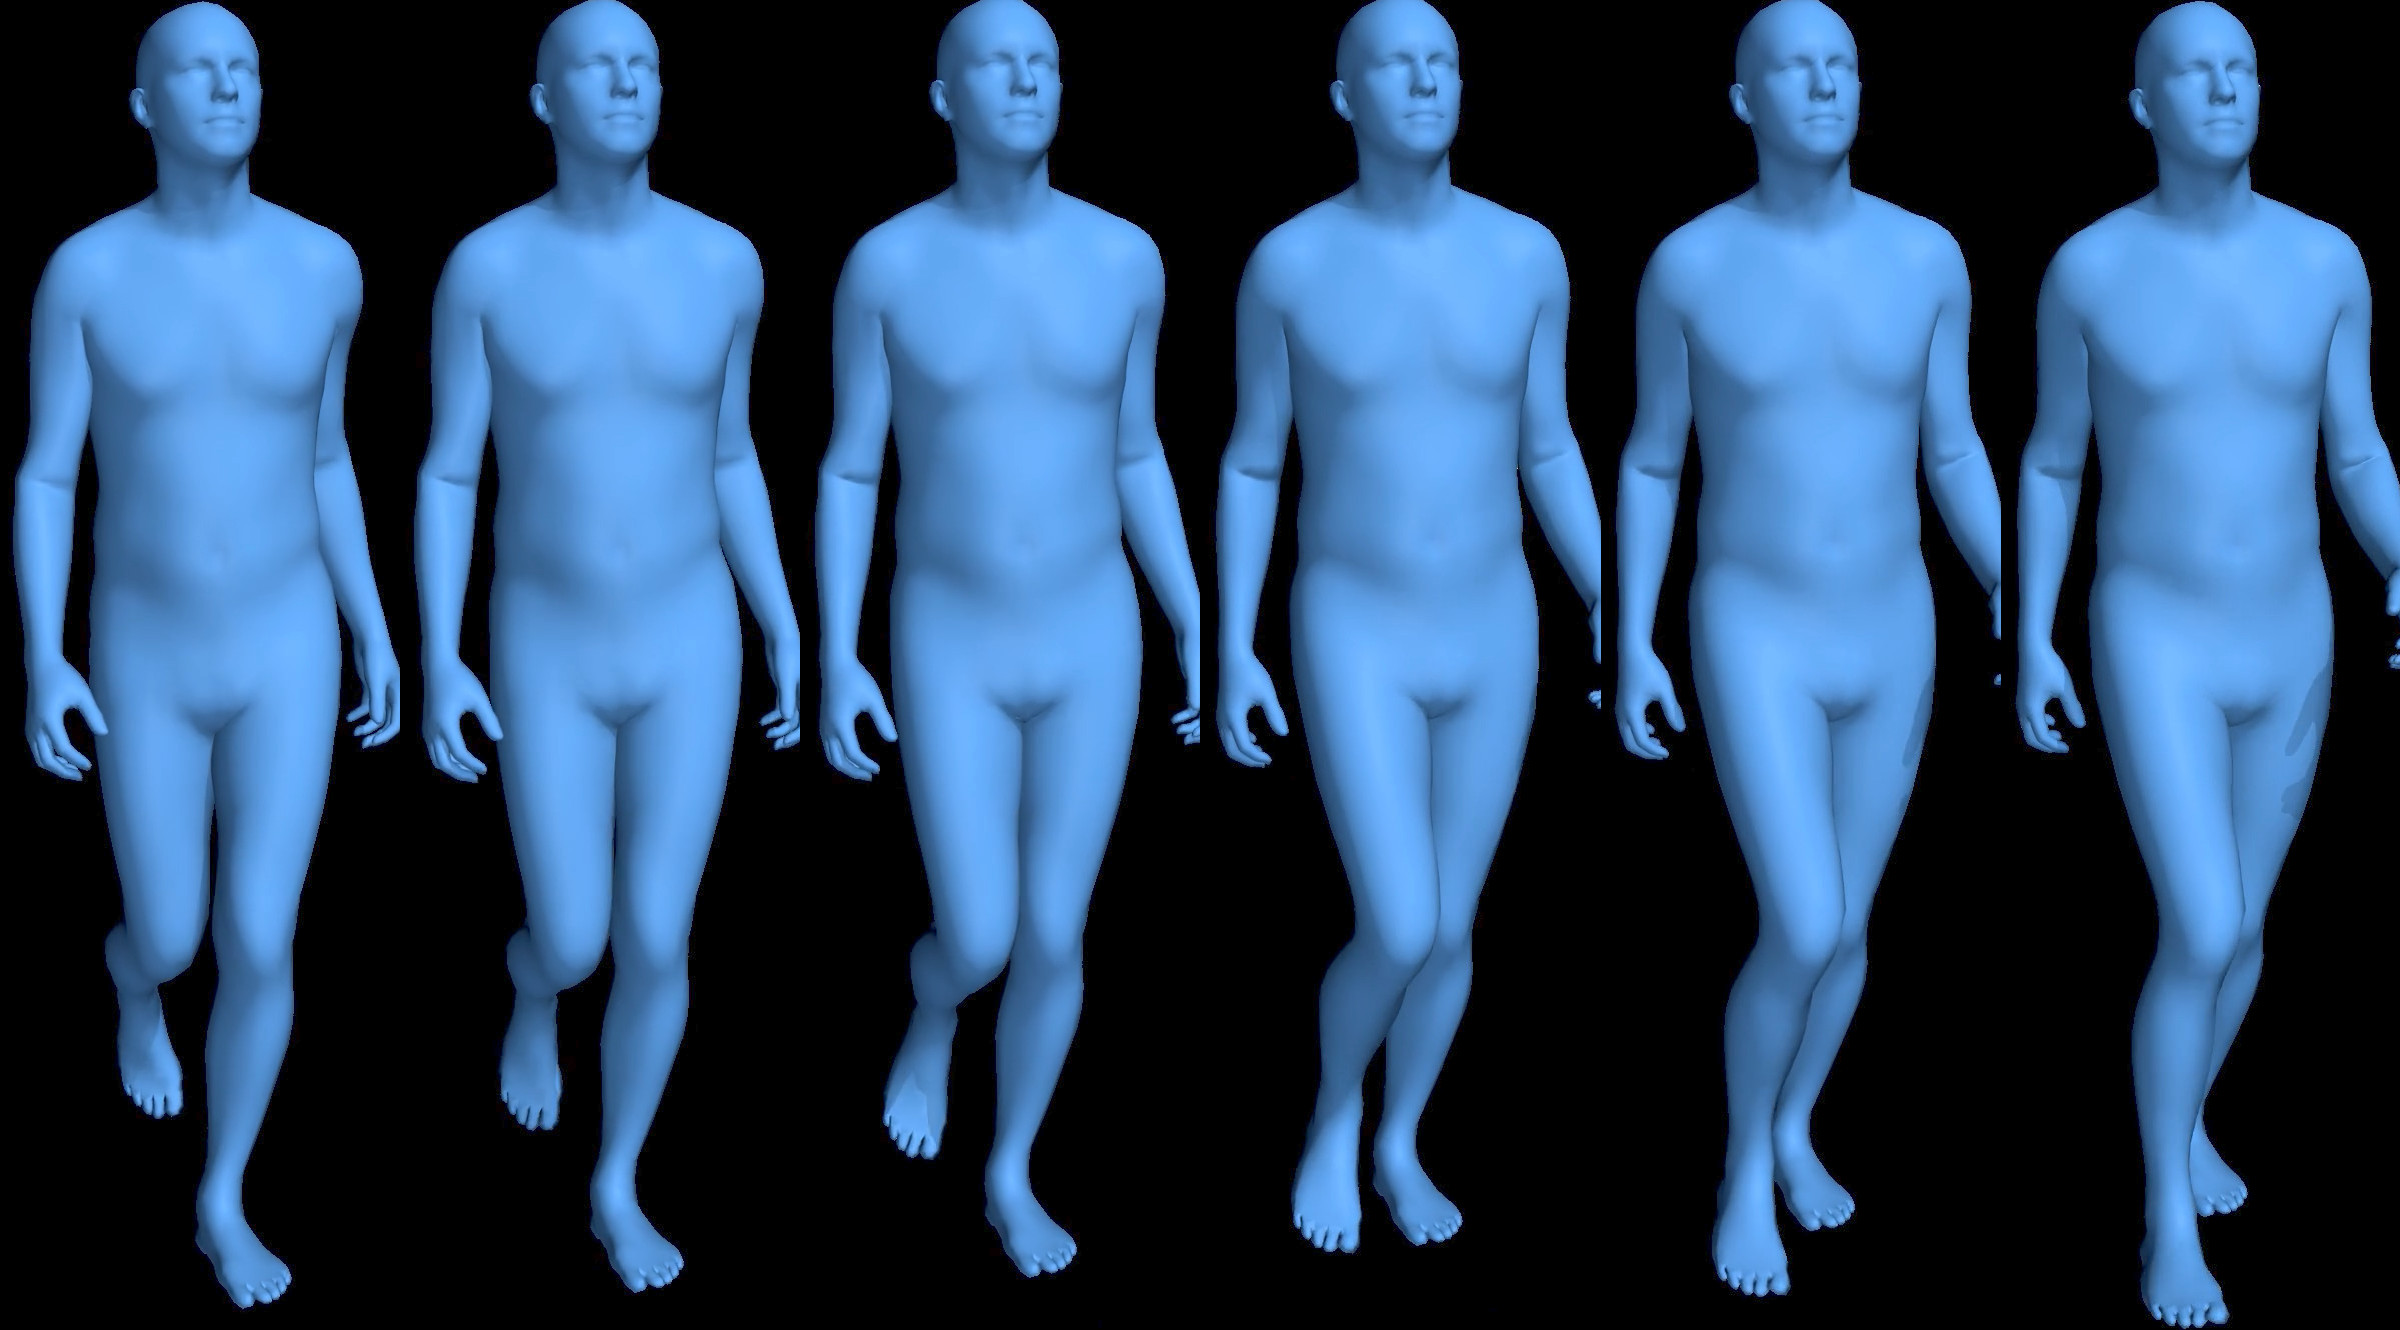
\includegraphics[width=0.3\textwidth]{img/02_01}
\caption{Small snippet of a walking motion from the AMASS dataset.}
\label{fig:walking}
\end{figure}




\subsection{Models}\label{subsec:models}
An autoencoder consists of an encoder and a decoder. The encoder works by taking an input and then encoding it into a smaller space called the latent space. The encoder then decodes the latent value back into something similar to the original input value. Such an operation by itself does not add any new information, but by doing this the model is forced to learn which features of the input are necessary for faithful reconstruction and which features can be discarded. This essentially gives us a compressed version of the input, where each change in the latent space is likely to be clearly visible in the output, similar to principal components analysis~\cite{shlens2014tutorial}.

Let $x$ denote the input, $e$ denote the encoder, $d$ denote the decoder, $z$ denote the latent value and $\hat{x}$ the autoencoded value, see \autoref{fig:autoencoder}. The following then needs to be minized
$$
\epsilon(x,\hat{x})
$$
where $\epsilon$ denotes the loss function~\cite{rocca2019understanding}.

Choosing to use the mean squared error (MSE) as the loss function gives
$$
\epsilon(x, \hat{x}) = \norm{x-\hat{x}}^2 = \norm{x-\mathrm{d}(\mathrm{e}(x))}^2
$$

Two models are constructed one with a small latent space and one with a large latent space. The models consist of a sequence of dense layers.

The model with a large latent space has a latent space with dimensions 4 and uses the following configuration of layers for its encoder $\abs{x} \to 1024 \to 64$, where each mapping happens in a dense layer and $\abs{x}$ denotes the input size.

The model with a small latent space has a latent space with dimensions 4 and uses the following configuration of layers for its encoder $\abs{x} \to 256 \to 256 \to 256 \to 256 \to 4$, where each mapping happens in a dense layer and $\abs{x}$ denotes the input size.

The decoderes of both models are mirrored versions of the encoders. Between each layer a Gaussian Error Linear Unit (GELU) \cite{hendrycks2020gaussian} is used as the activation function, with the exception of the last layer of the decoder. That layer is a linear layer.


\begin{figure}[h]
\centering
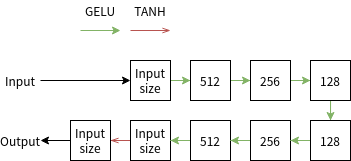
\includegraphics[width=0.5\textwidth]{img/autoencoder}
\caption{Diagram of the structure behind an autoencoder.}
\label{fig:autoencoder}
\end{figure}


An VAE is an autoencoder whose training is regularized \cite{rocca2019understanding}. This is achieved by altering the model architecture and the loss function.

Instead of encoding to a value in the latent space and passing that on to the decoder, the VAE encodes to a distribution in latent space. Decoding then happens by sampling this distribution and using that sample as the basis of decoding. This gives a latent distribution defined by $p(z \given x)$ and the sample is then $z \sim p(z \given x)$. Choosing a normal distribution as the latent distribution then yields $z \sim N(\mu, \sigma)$. This means that instead of encoding to a single value the encoder outputs a standard deviation and a mean.

The loss function can then be augmented with the Kullback–Leibler divergence (KLD) \cite{KLD} which measures relative entropy. The KLD is only dependent on the mean and variance which means that the loss function can be expressed as the MSE loss combined with the KLD loss.

$$
\begin{array}{c}
\mathrm{KLD} = -0.5 \sum{1 + \sigma_x - \mu_x^2 - \sigma_x^2} \\
\mathrm{MSE} = \norm{x-\mathrm{d}(\mathrm{e}(x))}^2 \\
\epsilon = \mathrm{KLD} + \mathrm{MSE}
\end{array}
$$

Minimizing on the KLD ensures regularization during the training process.

The VAE model is similar to the autoencoder with a small latent space. It has a latent space with dimensions 8 and uses the following configuration of layers for its encoder $\abs{x} \to 256 \to 256 \to 256 \to 256 \to 8$, where each mapping happens in a dense layer and $\abs{x}$ denotes the input size. In contrast to the autoencoder the VAE outputs two vectors of size 8, that correspond to $\mu$ and $\sigma$. Like the autoencoders GELU is the activation function for each layer, except the last which is linear.


\subsection{Training}\label{subsec:training}
The models were trained using the Adam optimizer \cite{kingma2017adam}.

Lower learning rates generally performed better, but increased the overall training time. As such a learning rate of \num{1e-5} was used for training all models.

A similar observation was made for the batch size, where generally speaking a lower batch size resulted in a lower loss, but after a much longer training time. The autoencoder with a large latent space was trained with batch size 128. The autoencoder with a small latent space and the VAE was trained with a batch size of 8.
